In questo capitolo viene presentato un excursus sulle varie fasi della progettazione e implementazione del database a grafo e dell'API RESTful. 
Per quanto riguarda la base di dati, ne viene descritta la struttura e ne vengono evidenziati i vantaggi. Inoltre vengono mostrate alcune delle query più importanti per l'implementazione del database, come quelle legate alla definizione delle relazioni tra le entità, oppure quelle utili al reperimento di dati, ad esempio quelli utilizzati dalle visualizzazioni di BITVAS.

L'approccio della trattazione dell'API è di tipo top-down, partendo con la definizione dell'architettura e del diagramma di comunicazione tra i vari moduli progettati, fino agli endpoint messi a disposizione dalla API e di conseguenza le funzionalità sviluppate.
Infine vengono descritti in modo più specifico i singoli moduli, evidenziandone tutte le particolarità.

\subsection{Struttura del Database}

Le entità principali delle visualizzazioni messe a disposizione da BITVAS sono quindi i flussi di Bitcoin tra blocchi o transazioni.
Questi ultimi sono oggetto di studi in diversi campi, partendo dalla cybesecurity, attraverso l'individuazione e la prevenzione di possibili pattern malevoli, fino ad arrivare a studi speculativi sul prezzo di Bitcoin.

L'analisi dei \emph{tempi di permanenza} (o in inglese \emph{holding time}) dei bitcoin all'interno dei portafogli degli utenti della rete \cite{holdingTimes} è uno degli aspetti fondamentali per questi tipi di valutazione, tramite i quali è possibile catalogare i vari tipi di holders.
Nonostante la necessità del supporto di strumenti statistici per comprenderne tutti i dettagli e le relazioni che li legano, la possibilità di sviluppo di altre visualizzazioni per BITVAS, in grado di dare un'anteprima visuale su tali holding times e il bisogno di semplificare l'interpretazione della grande mole di dati presenti nella blockchain, ha portato allo sviluppo della seguente base di dati a grafo, tramite la quale è possibile gestire il gran numero di relazioni tra le informazioni in modo più efficiente ed efficace.
\newpage
\thispagestyle{mystyle}
\begin{figure}[H]
    \centering 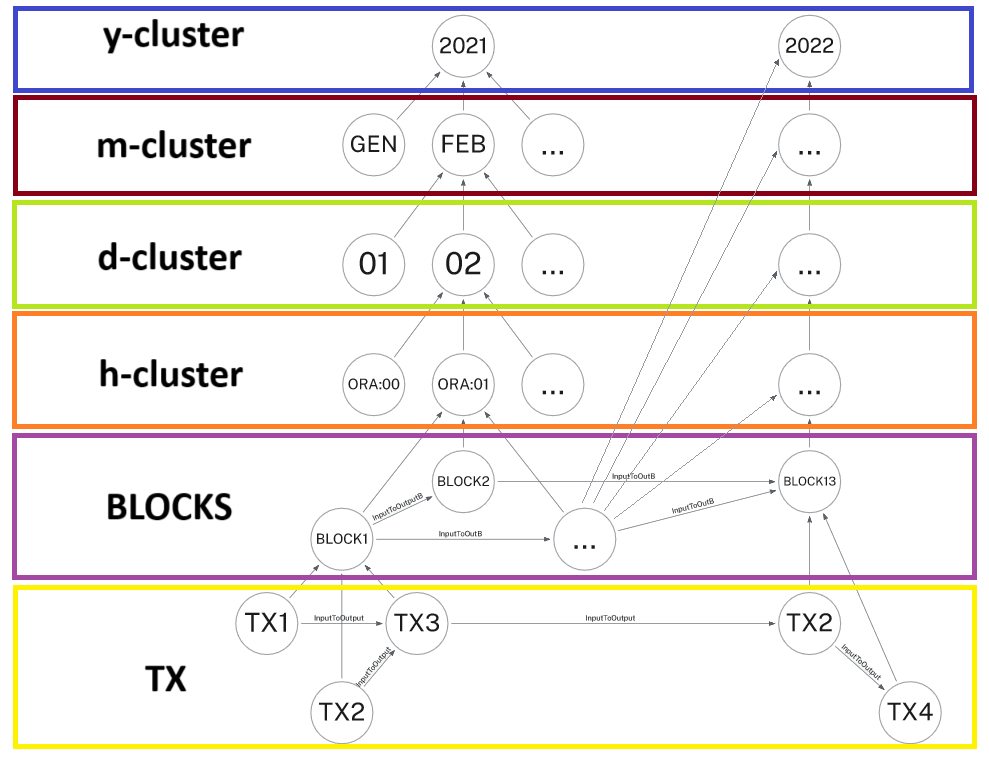
\includegraphics[keepaspectratio=true,scale=0.58]{Images/ExampleDB.png}
    \caption{Rappresentazione concettuale ed estesa del database a grafo}
\end{figure}

In figura 5 è rappresentato il database di riferimento.
La struttura è di tipo \emph{time-tree} (in italiano, albero temporale), alla cui base si trovano le entità fondamentali corrispondenti a quelle utilizzate nella blockchain di Bitcoin, ovvero blocchi e transazioni.
Ognuna delle quali possiede attributi in grado di fornirne i dettagli, tra cui quelli utilizzati per la loro identificazione univoca, come \textit{id} per blocchi o \textit{hash} per le transazioni.

Come già trattato, la blockchain al giorno d'oggi fa riferimento ad una grande quantità di informazioni, legati anche ai flussi di Bitcoin.
Per rendere più efficiente l'estrapolazione dei dati nei casi in cui si voglia tener conto di flussi che partono o arrivano ad un determinato insieme di blocchi, appartenenti ad un definito arco temporale ed evitare un'analisi dispendiosa  al livello di blocco o transazione, si è deciso di progettare più livelli di clusterizzazione.

Il livello successivo ai blocchi è dato dagli \emph{h-cluster} (hour-cluster), che fanno riferimento ai blocchi minati in una determinata ora, ovvero circa sei.
Salendo nella struttura si incontrano, nel seguente ordine, i \emph{d-cluster} (day-cluster), \emph{m-cluster} (month-cluster) e \emph{y-cluster} (year-cluster).

Il tipo di struttura, in grado di facilitare la ricerca tramite \emph{timestamp}, è definita dalle relazioni gerarchiche,
nel caso in cui un nodo di livello inferiore faccia parte di uno dei cluster superiori.
Un esempio di relazione gerarchica è quella tra transazioni e blocchi o tra blocchi e h-cluster. 
Con l'utilizzo di attributi come \emph{minimum} e \emph{maximum}, che rappresentano rispettivamente l'id minimo e massimo dei blocchi a cui fa riferimento il cluster, anche la ricerca tramite id viene valorizzata dal database.
Inoltre per facilitare il reperimento dei flussi di Bitcoin che riguardano cluster di livello diverso, ognuno di essi, all'occorrenza, ha una relazione con tutti gli altri cluster verso il quale spende Bitcoin, la quale contiene informazioni riguardante il volume di valuta scambiato, attraverso due parametri, ovvero \emph{value} e \emph{value$\_$usd}.

Di seguito viene mostrato il modello completo della base di dati, con tutti i nodi e le relazioni presenti al suo interno.

\thispagestyle{mystyle}

\begin{figure}[H]
    \centering 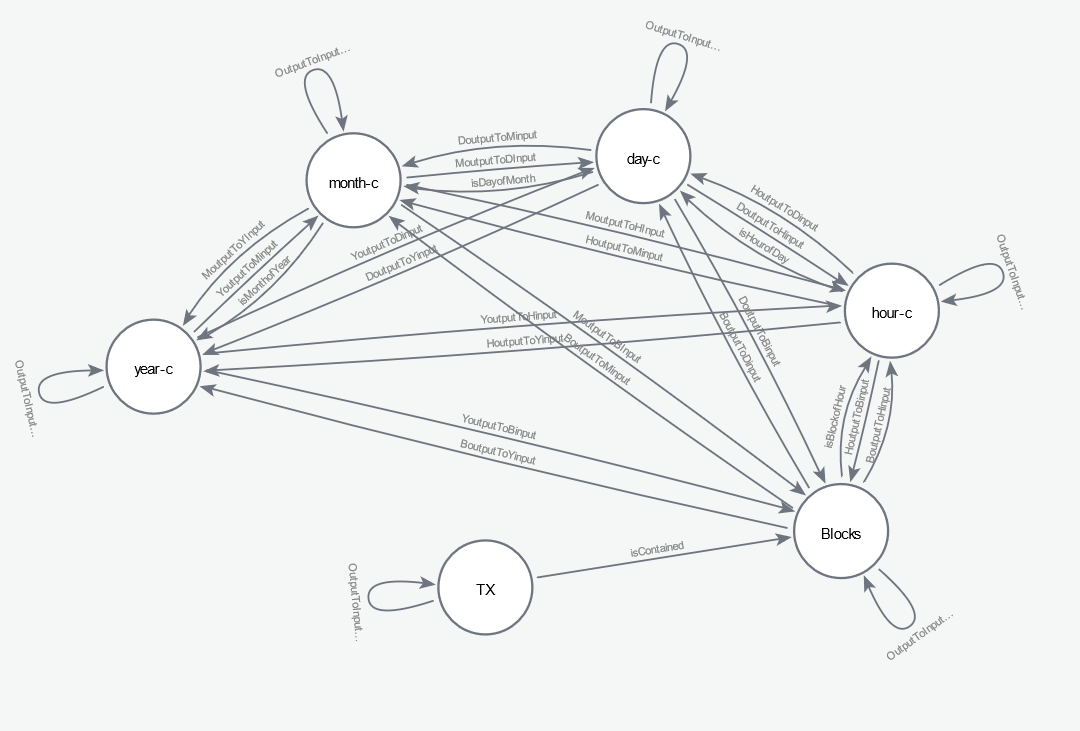
\includegraphics[keepaspectratio=true,scale=0.52]{Images/Modello completo.png}
    \caption{Modello completo del database a grafo}
\end{figure}
Per evidenziare il collegamento di una transazione con un blocco viene fatto riferimento alla relazione \emph{isContained}, mentre per le altre gerarchie viene utilizzato lo schema nominativo \emph{isXofY}.
I flussi di Bitcoin invece sono definiti dalle relazioni \emph{XOutputToYInput}.
Per entrambi i tipi, al posto di X e Y vanno sostituiti i cluster a cui si fa riferimento.
Se un flusso si riferisce a due nodi appartenenti alla stessa tipologia di nodo, la nomenclatura utilizzata è \emph{OutputToInputX}.
Ad esempio per i blocchi la relazione che identifica i flussi è \emph{OutputToInputB}.
Le relazioni che partono e arrivano alla stesso nodo si riferiscono agli scambi di cryptovaluta che avvengono nello stesso arco temporale definito dal cluster di riferimento.
Ad esempio una autorelazione di un blocco, sta ad indicare la presenza di un flusso di Bitcoin tra due transazioni validate al suo interno.

Il database implementato prevede all'incirca due milioni e mezzo di nodi e quattro milioni di relazioni, strutturate come segue:



\begin{center}
\begin{tabular}{|c|c|c|}
\hline
 LISTA BLOCCHI & LISTA TRANSAZIONI & FILE INPUT.CSV \\ 
 \hline
 2023-12-07 & 2023-12-07 & 2023-12-20 \\ 
  to & 2023-12-18 & 2024-01-05 \\
  2024-01-07 & 2023-12-20 & \\
   & 2024-01-04 & \\
   & 2024-01-05 & \\
 \hline
\end{tabular}

\end{center}
\thispagestyle{mystyle}
L'insieme dei dati è stato estrapolato dal dataset messo a disposizione su Blockchair.com \cite{blockchair}. I file INPUT.CSV sono quelli utili per la definizione delle relazioni che rappresentano i flussi di Bitcoin.

\subsubsection{Query per la definizione della struttura}
Di seguito vengono mostrate le Cypher Query più importanti utilizzate per la definizione della struttura della base di dati.

\begin{center}
Creazione dei nodi Transaction
   \begin{lstlisting}

            LOAD CSV WITH HEADERS FROM 'file:///TX.csv'
            AS row WITH split(row.time,' ')AS date, row
            MERGE (:Transaction {block_id: row.block_id, 
                   hash: row.hash,
                   input_count: row.input_count,
                   output_count: row.output_count, 
                   input_total: row.input_total, 
                   input_total: row.input_total,  
                   output_total: row.output_total, 
                   fee: row.fee,
                   is_coinbase: row.is_coinbase})
\end{lstlisting} 
\end{center}
Con i dati presenti nel file TX.csv vengono inizializzati i nodi che rappresentano le transazioni all'interno della base di dati, con i relativi attributi.
\newpage \thispagestyle{mystyle}
\begin{center}
Creazione dei nodi Blocks
   \begin{lstlisting}

            LOAD CSV WITH HEADERS FROM 'file:///Blocchi.csv'
            AS row WITH split(row.time, ' ') AS date ,row
            MERGE (:Blocks {id: row.id, hash: row.hash, 
                    time:   datetime(date[0]+'T'+date[1]+'Z'),
                    transaction_count: row.transaction_count, 
                    input_count: row.input_count, 
                    output_count: row.output_count,
                    input_total: row.input_total,  
                    output_total: row.output_total, 
                    fee_total: row.fee_total,
                    guessed_miner: row.guessed_miner})
\end{lstlisting} 
\end{center}
 Con questa query vengono inseriti i nodi rappresentativi dei blocchi all'interno del database con i relativi attributi estratti dal file Blocchi.csv.
 
 Per la costruzioine delle relazioni tra transazioni e blocchi, e quindi generare una sorta di grafo delle transazioni, vengono utilizzate le seguenti query, che usufruiscono dei dati presenti nei file INPUT.csv.

\vspace{5mm}
\begin{center}
Creazione delle relazioni tra blocchi
   \begin{lstlisting}

            LOAD CSV WITH HEADERS FROM 'file:///IN_20240105.csv' AS row
            MATCH (b:Blocks {id:row.block_id}), 
                  (b2:Blocks {id:row.spending_block_id})
            MERGE  (b)-[ib:inputToOutputB]->(b2)
            SET (ib.block_id=row.block_id, 
                ib.spending_block_id=row.spending_block_id, 
                ib.value=row.value,
                ib.is_from_coinbase = row.is_from_coinbase, 
                ib.is_spendable= row.is_spendable, 
                ib.value_usd = row.value_usd)
\end{lstlisting} 
\end{center}
\newpage \thispagestyle{mystyle}
\begin{center}
Creazione delle relazioni tra transazioni
\begin{lstlisting}

            LOAD CSV WITH HEADERS FROM 'file:///IN_20240105.csv' AS row
            MATCH (t:Transactions {hash:row.transaction_hash}), 
                  (t2:Transactions{hash:row.spending_transaction_hash})
            MERGE  (t)-[i:inputToOutputTX]->(t2)
            SET i.transaction_hash=row.transaction_hash,
                i.spending_TX_hash=row.spending_TX_hash,
                i.value=row.value,
                i.value_usd = row.value_usd,
                i.is_from_coinbase = row.is_from_coinbase
\end{lstlisting} 
\end{center}
 Nelle seguenti query viene mostrata la definizione degli altri cluster progettati a partire dall'attributo time dei nodi appena inseriti, estrapolandone le porzioni necessarie (es. per i day-cluster vengono estratti anno,mese e giorno).
\vspace{5mm}
\begin{center}
Creazione dei nodi Hour-Cluster
   \begin{lstlisting}

            MATCH(b:Blocks)  
            WITH DISTINCT (b.time.year 
                            + '-' + b.time.month 
                            + '-' + b.time.day 
                            + 'T' + b.time.hour) AS IDHour
            CREATE (h:hCluster{htime:IDHour})
\end{lstlisting} 
\end{center}
\vspace{3mm}
 \begin{center}
Creazione dei nodi Day-Cluster

   \begin{lstlisting}
            MATCH(b:Blocks)  
            WITH DISTINCT (b.time.year 
                            + '-' + b.time.month 
                            + '-' + b.time.day) AS IDDay
            CREATE (d:dCluster{dtime:IDDay})
\end{lstlisting} 
\end{center}

\newpage \thispagestyle{mystyle}

 \begin{center}
Creazione dei nodi Month-Cluster
   \begin{lstlisting}

            MATCH(b:Blocks)  
            WITH DISTINCT (b.time.year 
                            + '-' + b.time.month) AS IDMonth
            CREATE (m:mCluster{mtime:IDMonth})
\end{lstlisting} 
\end{center}
\vspace{2mm}
\begin{center}
Creazione dei nodi Year-Cluster
   \begin{lstlisting}

            MATCH(b:Blocks)  
            WITH DISTINCT (b.time.year) AS IDYear
            CREATE (y:yCluster{ytime:IDYear})
\end{lstlisting} 
\end{center}


Dopo aver definito tutte le entità appartenenti alla base di dati, sono state definite le relazioni gerarchiche che legano i vari cluster e successivamente gli attributi di questi ultimi. Le strutture di quest'ultime sono molto simili tra loro con qualche piccola differenza in base al cluster a cui si fa riferimento. Di seguito sono mostrate le query usate per la gestione degli Hour-Cluster.

\vspace{5mm}
\begin{center}
Creazione relazioni tra blocchi e Hour-Cluster
\begin{lstlisting}

            MATCH (b:Blocks),(h:hCluster)  
            WHERE h.htime = b.time.year 
                    + '-' + b.time.month
                    + '-' + b.time.day 
                    + 'T' + b.time.hour
                    
            MERGE (b)-[i:isBofH]->(h)
\end{lstlisting} 
\end{center}
\vspace{2mm}
\begin{center}
Inizializzazione attributi degli Hour-Cluster
\begin{lstlisting}

            MATCH (b:Blocks)-[r:isBofH]->(h:hCluster) 
            WITH DISTINCT h,
                    sum(toInteger(b.input_total)) AS total_h_input,
                    sum(toInteger(b.output_total)) AS total_h_output

            MERGE (b)-[i:isBofH]->(h)
\end{lstlisting} 
\end{center}
\newpage \thispagestyle{mystyle}
In seguito alla definizione di tutti i cluster e delle relazioni gerarchiche, la struttura del database assume la forma di un albero temporale, tramite il quale le query di ricerca tramite timestamp risultano molto efficaci.
Le query per l'inizializzazione delle relazioni identificative dei flussi di Bitcoin sono di due tipi, quelle riguardanti lo stesso tipo di cluster o meno.
Quest'ultime hanno una struttura molto simile per ogni cluster.
Di seguito vengono mostrate quelle utilizzate per la creazione di quelle riguardanti i flussi il cui punto di partenza sono gli Hour-Cluster.
\vspace{5mm}
\begin{center}
Inizializzazione relazioni tra i nodi Hour-Cluster
\begin{lstlisting}

           MATCH (b:Blocks)-[ih:isBofH]->(h:hCluster),
                    (b2:Blocks)-[ih2:isBofH]->(h2:hCluster), 
                    (b)-[ib:inputToOutputB]->(b2)
            WITH DISTINCT h,h2,sum(toInteger(ib.value))AS hClusterFlow, 
                          sum(toFloat(ib.value_usd))AS hClusterFlowUSD
                          
            MERGE (h)-[ih:inputToOutputH]->(h2)
            SET ih.value = hClusterFlow,
                ih.value_usd = hClusterFlowUSD

\end{lstlisting} 
\end{center}

\vspace{5mm}
\begin{center}
Inizializzazione relazioni tra Hour-Cluster e Year-Cluster
\begin{lstlisting}

            MATCH (h2:hCluster)-[io:inputToOutputH]->
                    (h:hCluster)-[ih:isHofD]->
                    (d:dCluster)-[id:isDofM]->
                    (m:mCluster)-[i:isMofY]->
                    (y:yCluster) 
            WITH h2,y,sum(io.value) AS value, 
                 sum(io.value_usd) AS value_usd
                
            MERGE (h2)-[ib:HOutputToYInput]->(y)
            SET ib.value = value, 
                ib.value_usd = value_usd

\end{lstlisting} 
\end{center}

\vspace{5mm}
\newpage \thispagestyle{mystyle}
\begin{center}
Inizializzazione relazioni tra Hour-Cluster e Blocks
\begin{lstlisting}

            MATCH (b2:Blocks)-[io:inputToOutputB]->
                  (b:Blocks)-[iblock:isBofH]->(h:hCluster),
                  (b2)-[iblock2:isBofH]->(h2:hCluster)
            WHERE b2.time <> b.time
            WITH h2,b,io,sum(io.value) AS value,
                 sum(io.value_usd) AS value_usd
                
            MERGE (h2)-[ioy:HOutputToBInput]->(b)
            SET  ioy.value = value, 
                 ioy.value_usd = value_usd

\end{lstlisting} 
\end{center}
\vspace{3mm}
\begin{center}
Inizializzazione relazioni tra Hour-Cluster e Day-Cluster
\begin{lstlisting}

            MATCH (h2:hCluster)-[io:inputToOutputH]->
                  (h:hCluster)-[ih:isHofD]->(d:dCluster)
            WITH h2,d,sum(io.value) AS value, 
                 sum(io.value_usd) AS value_usd

            MERGE (h2)-[ib:HOutputToDInput]->(d)
            SET ib.value = value, 
                ib.value_usd = value_usd

\end{lstlisting} 
\end{center}

\vspace{3mm}
\begin{center}
Inizializzazione relazioni tra Hour-Cluster e Month-Cluster
\begin{lstlisting}

            MATCH (h2:hCluster)-[io:inputToOutputH]->
                  (h:hCluster)-[ih:isHofD]->
                  (d:dCluster)-[id:isDofM]->(m:mCluster)
            WITH h2,m,sum(io.value) AS value, 
                 sum(io.value_usd) AS value_usd

            MERGE (h2)-[ib:HOutputToMInput]->(m) 
            SET ib.value = value, 
                ib.value_usd = value_usd
\end{lstlisting} 
\end{center}
\newpage \thispagestyle{mystyle}
Per permettere la ricerca dei blocchi anche tramite id e non solo tramite timestamp, sono stati aggiunti due parametri ai cluster, ovvero minimum e maximum che indicano rispettivamente l'id minimo e massimo a cui fa riferimento.
Questi vengono definiti con le seguenti query.

\vspace{3mm}
\begin{center}
Inizializzazione minimum e maximum per gli Hour-Cluster
\begin{lstlisting}

            MATCH (b:Blocks)-[r:isBofH]->(h:hCluster)
            WITH  h,
                  MIN(b.id)AS MINIMUM,
                  MAX(b.id) AS MAXIMUM
                  
            SET   h.mimimum = MINIMUM,
                  h.maximum = MAXIMUM
\end{lstlisting} 
\end{center}

\vspace{3mm}
\begin{center}
Inizializzazione minimum e maximum per i Day-Cluster
\begin{lstlisting}

            MATCH (h:hCluster)-[r:isHofD]->(d:dCluster)
            WITH  d,
                  MIN(h.minimum)AS MINIMUM,
                  MAX(h.maximum) AS MAXIMUM
                  
            SET   d.mimimum = MINIMUM,
                  d.maximum = MAXIMUM
\end{lstlisting} 
\end{center}

Le query per la definizione di questi attributi per gli altri cluster sono uguali a quest'ultima con adeguato adattamento delle entità prese come riferimento.

\subsubsection{Query per il reperimento di dati}
La struttura generata assume di conseguenza la forma di un time-tree i cui nodi sono legati da relazioni che rappresentano i flussi di Bitcoin, tramite la quale è possibile etrarre i dati necessari per le visualizzazioni di BITVAS e non solo, in maniera semplice, veloce ed efficace.
Infatti la ricerca di un determinato nodo tramite timestamp, o id nel caso dei blocchi risulta fortemente migliorata, in quanto non è necessaria la verifica di tutti i nodi,ma viene effettuata seguendo la struttura ad albero. 
Di seguito vengono mostrate le query utilizzate dall'API per permettere un'interazione con il database.

\newpage \thispagestyle{mystyle}

\begin{center}
Flussi tra Day-Cluster
\begin{lstlisting}

            MATCH (d:dCluster)-[im:isDofM]->
                  (m:mCluster)-[iy:isMofY]->(y:yCluster)
            WHERE y.ytime = '2024' AND m.mtime = '2024-01'
                  AND d.dtime = '2024-01-05'
            WITH d

            MATCH (d2)-[io:inputToOutputD]->(d)
            WHERE d2.dtime >= '2023-12-10' 
                  AND d2.dtime <='2023-12-20' 
            RETURN d2.dtime,d.dtime,io.value,io.value_usd
\end{lstlisting} 
\end{center}

La prima parte della query permette di individuare il cluster di arrivo attraverso la struttura ad albero, il quale viene utilizzato successivamente per selezionare tutti i flussi che arrivano ad esso e che partono da un insieme di day-cluster definiti tramite un arco temporale ben definito.

\vspace{5mm}
\begin{center}
Flussi da Hour-Cluster a Day-Cluster 
\begin{lstlisting}

            MATCH (d:dCluster)-[id:isDofM]->
                  (m:mCluster)-[im:isMofY]->(y:yCluster)
            WHERE y.ytime = '2024' 
                  AND m.mtime = '2024-01' 
                  AND d.dtime='2024-01-05'
            WITH d

            MATCH (h:hCluster)-[rels:HOutputToDInput]->(d)
            WHERE h.htime >='2023-12-10T02' 
                  AND h.htime <= '2023-12-20T04' 
            RETURN  h.htime,rels.value,rels.value_usd,d.dtime
\end{lstlisting} 
\end{center}

In questo caso vengono prelevati tutti i flussi che hanno come punto di partenza gli hour-cluster definiti dall'arco temporale scelto e come punto di arrivo il day-cluster selezionato.

Oltre a query strettamente legate ai flussi di Bitcoin è possibile anche prelevare gli attributi delle entità all'interno del database e quindi ottenere delle informazioni generali. In seguito viene mostrato un esempio di quest'ultime.

\newpage \thispagestyle{mystyle}

\begin{center}
Ottenimento informazioni dei blocchi
\begin{lstlisting}

            MATCH (b:Blocks)-[i:isBofH]->
                  (h:hCluster)-[ih:isHofD]->
                  (d:dCluster)-[id:isDofM]->
                  (m:mCluster)-[im:isMofY]->(y:yCluster)
            WHERE y.ytime = '2024'  
                  AND m.mtime = '2024-01' 
                  AND d.dtime = '2024-01-05' 
                  AND h.htime = '2024-01-05T02'
                  AND b.time = '2024-01-05T02:47:03'
            RETURN b.id,toString(b.time),b.hash,
                   b.guessed_miner,b.fee_total,
                   b.output_count,b.input_count,b.output_total,
                   b.input_total, b.transaction_count 
                   ORDER BY b.time
\end{lstlisting} 
\end{center}
\vspace{5mm}
\begin{center}
Ottenimento informazioni dei Month-Cluster
\begin{lstlisting}

            MATCH MATCH (m:mCluster)-[im:isMofY]->(y:yCluster)
            WHERE y.ytime = '2024'  
                  AND m.mtime = '2024-01'
            RETURN m.mtime,m.minimum,m.maximum,
                   m.total_m_input,m.total_m_output
                   ORDER BY m.mtime
\end{lstlisting} 
\end{center}

La struttura della query per l'estrazione dei dati riguardanti gli altri cluster è pressochè identica.
Si parte con l'individuazione tramite la struttura ad albero, dopodichè si estraggono i corrispondenti dati.

Come trattato in precedenza il focus dello sviluppo dell'API e del database si basa sull'interazione di quest'ultimo con BITVAS. Di seguito vengono mostrate le query utili al reperimento dei dati per le visualizzazioni già esistenti.

\newpage \thispagestyle{mystyle}

\begin{center}
Ottenimento prima parte della BlockVisualization
\begin{lstlisting}

            WITH datetime('2024-01-05T09:43:19Z') - duration('PT12H') 
                 AS firstTwelveT
            MATCH  (b:Blocks)-[i:isBofH]->
                   (h:hCluster)-[ih:isHofD]->
                   (d:dCluster)-[id:isDofM]->
                   (m:mCluster)-[im:isMofY]->(y:yCluster)
            WHERE y.ytime = '2024' AND m.mtime ='2024-01'  
                  AND d.dtime ='2024-01-05' 
                  AND h.htime  = '2024-01-05T09' 
                  AND b.time=datetime('2024-01-05T09:43:19Z')
            With b, firstTwelveT
            
            MATCH (h)-[i:inputToOutputB]->(b)
            WHERE h.time >= firstTwelveT AND h.time<= b.time
            RETURN h.id,h.time,b.id,b.time ORDER BY h.time
\end{lstlisting} 
\end{center}
La BlockVisualization pone il focus su un determinato blocco e i flussi di Bitcoin che arrivano e partono da esso.
In questo caso vendono estrapolati i dati identificativi dei flussi che partono da blocchi il cui timestamp è compreso nelle dodici ore precedenti e arrivano blocco scelto.

\begin{center}
Ottenimento seconda parte della BlockVisualization
\begin{lstlisting}
            WITH datetime('2024-01-05T09:43:19Z') + duration('PT12H') 
                 AS secondTwelveT
            MATCH  (b:Blocks)-[i:isBofH]->
                   (h:hCluster)-[ih:isHofD]->
                   (d:dCluster)-[id:isDofM]->
                   (m:mCluster)-[im:isMofY]->(y:yCluster)
            WHERE y.ytime = '2024' AND m.mtime ='2024-01'  
                  AND d.dtime ='2024-01-05' 
                  AND h.htime  = '2024-01-05T09' 
                  AND b.time=datetime('2024-01-05T09:43:19Z')
            With b, secondTwelveT 
            
            MATCH (b)-[i:inputToOutputB]->(h) 
            WHERE h.time <= secondTwelveT AND h.time > b.time  
            RETURN b.id,b.time,h.id,h.time ORDER BY h.time
\end{lstlisting} 
\end{center}
\newpage \thispagestyle{mystyle}
La struttura è molto simile alla prima, con qualche piccola diffenza legata al punto di partenza dei flussi, che in questo caso è il blocco centrale della visualizzazione. Mentre il punto di arrivo sono i blocchi il cui timestamp è compreso nelle dodici ore successive al blocco selezionato.
L'insieme delle due permettono l'estrapolazione necessaria per ottenere l'intera visualizzazione.

Anche la TransactionVisualization `e divisa in due parti, mostrate di seguito.
\begin{center}
Ottenimento prima parte della Transaction Visualization
\begin{lstlisting}
            WITH  hash AS chosenTX
            MATCH (t:Transactions)
            WHERE t.hash = chosenTX
            WITH t

            MATCH (t)-[r:inputToOutputTX]->(c)
            RETURN t.hash as hash, t.block_id as blockStart, 
                   c.hash as hashEnd, c.block_id as blockEnd, 
                   r.value as value, r.value_usd as value_usd 
                   ORDER BY c.block_id
\end{lstlisting} 
\end{center}
\vspace{5mm}
\begin{center}
Ottenimento seconda parte della TransactionVisualization
\begin{lstlisting}
            WITH  hash AS chosenTX
            MATCH (t:Transactions)
            WHERE t.hash = chosenTX
            WITH t

            MATCH (c)-[r:inputToOutputTX]->(t)
            RETURN t.hash as hash, t.block_id as blockStart, 
                   c.hash as hashEnd, c.block_id as blockEnd, 
                   r.value as value, r.value_usd as value_usd 
                   ORDER BY c.block_id
\end{lstlisting} 
\end{center}
Una volta identificata la transazione, tramite hash, all'interno del database, si individuano le relazioni che partono e arrivano ad essa corrispondenti ai flussi di Bitcoin in ingresso e in uscita.

Per quanto riguarda la MinerVisualization e la CombinedVisualization per l'estrapolazione dei blocchi da visualizzare viene utilizzata un'interrogazione che può essere identificata come `Query di ricerca' mostrata di seguito.
\newpage \thispagestyle{mystyle}
\begin{center}
Query di ricerca
\begin{lstlisting}[basicstyle = \small]
            WITH toString(datetime('2024-01-05T09:43:19Z') 
                    - duration('PT12H')) AS firstTwelveT,
                 toString( datetime('2024-01-05T09:43:19Z') 
                 + duration('PT12H')) AS secondTwelveT
            WITH  split(firstSplit[0],'-') AS firstDate,
                  split(firstSplit[1],':') AS firstTime,
                  split(secondSplit[0],'-') AS secondDate,
                  split(secondSplit[1],'-') AS secondTime
                  
            MATCH  (b:Blocks)-[i:isBofH]->
                   (h:hCluster)-[ih:isHofD]->
                   (d:dCluster)-[id:isDofM]->
                   (m:mCluster)-[im:isMofY]->(y:yCluster)
            WHERE  y.ytime >= firstDate[0] AND y.ytime <= secondDate[0] 
                   AND m.mtime >= firstDate[0] + '-' + firstDate[1] 
                   AND m.mtime <= secondDate[0] + '-' + secondDate[1] 
                   AND d.dtime >= firstDate[0] + '-' + firstDate[1] 
                                  + '-' + firstDate[2]
                   AND  d.dtime <= secondDate[0] + '-' + secondDate[1] 
                                  + '-' + secondDate[2]
                   AND  h.htime >= firstDate[0] + '-' + firstDate[1] 
                                    + '-' + firstDate[2] +'T'+ 
                                    firstTime[0]
                   AND h.htime <= secondDate[0] + '-' + secondDate[1] 
                                    + '-' + secondDate[2] + 'T' + 
                                    secondTime[0]
                   AND b.time >= (datetime('2024-01-05T09:43:19Z') 
                                - duration('PT12H'))
                   AND b.time<= ( datetime('2024-01-05T09:43:19Z') 
                                + duration('PT12H'))
            WITH collect(b) as blocchi, collect(ID(b)) as listBlocks
\end{lstlisting} 
\end{center}

Tramite quest'ultima vengono estratti tutti i blocchi il cui timestamp è compresto nelle dodici ore precedenti e successive al timestamp del blocco centrale alla visualizzazione.
Per la MinerVisualization c'è una leggera differenza, ovvero un vincolo sul miner oltre a quelli temporali.
Le collezioni di blocchi ricavate vbengono utilizzate nella successiva subquery per l'estrapolazione dei flussi.
\newpage \thispagestyle{mystyle}

\begin{center}
Estrapolazione flussi tra i blocchi estratti per la MinerVisualization e la BlockVisualization
\begin{lstlisting}
           CALL{
                  WITH blocchi,listBlocks
                  UNWIND blocchi as x
                  MATCH (x)-[r:inputToOutputB]->(c)
                  WHERE ID(c) in listBlocks
                  RETURN x,c
            }
            RETURN x.id,x.time,c.id,c.time

\end{lstlisting} 
\end{center}

\subsection{Struttura dei JSON} 
Per la definizione delle visualizzazioni implementate in BITVAS si fa uso di file JSON, adeguatamente strutturati ai fini di ognuna di esse.
La corretta comprensione di questi ultimi è necessaria per garantire la corretta interazione tra BITVAS e il database a grafo, messa in atto dall'API RESTful sviluppata.

\begin{figure}[H]
    \centering 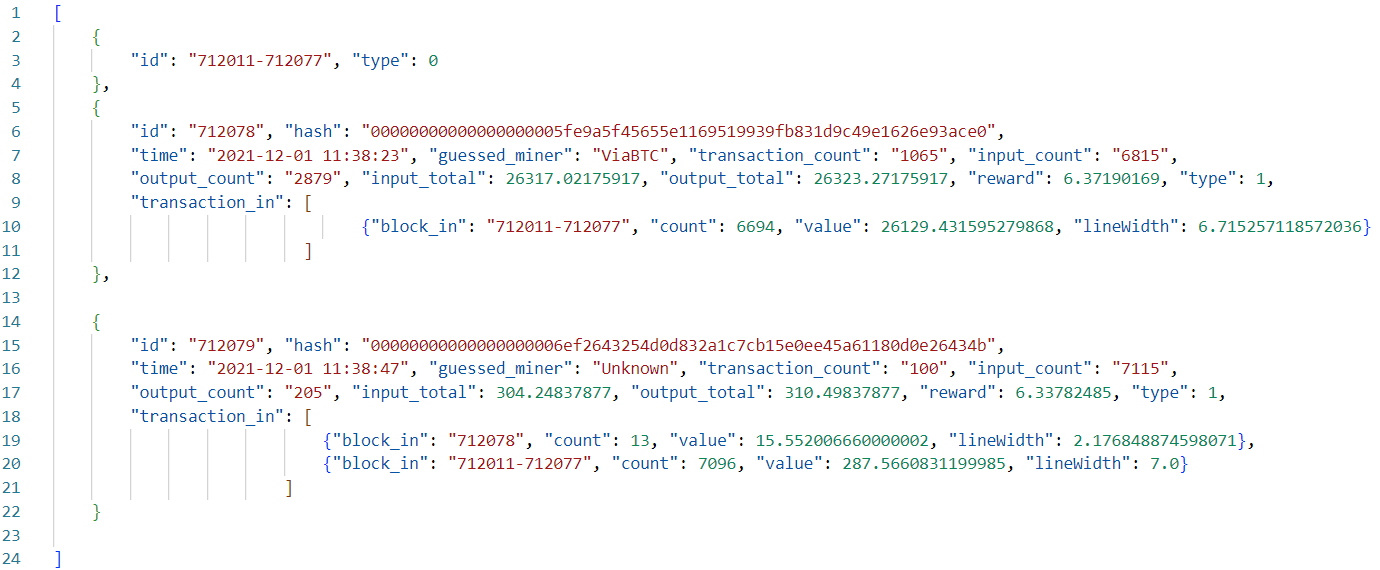
\includegraphics[keepaspectratio=true,scale=0.4]{Images/StrutturaJSON_BITVAS.png}
    \caption{Struttura del JSON usato da BITVAS per la visualizzazione iniziale}
\end{figure}

La totalità delle visualizzazioni di BITVAS pone il focus sui flussi di Bitcoin dei blocchi o delle transazioni visualizzate.
Ogni elemento del file corrisponde ad un'entità rappresentata dal software, la cui differenziazione viene gestita tramite il parametro \emph{type}, il quale può essere inizializzato con tre interi, ovvero zero, uno e due che indicano rispettivamente i cluster block, blocchi e transazioni.
In figura 7 vengono mostrate solo le prime due entità elencate.
I cluster block sono identificati da un id che contiene il range dei blocchi da cui è formato e da type.
Invece per quanto riguarda i blocchi, oltre all' id, vengono inizializzati una serie di parametri utili a fornire dettagli su di essi, tra cui \textit{guessed$\_$miner} utilizzato per identificare il miner che lo ha validato, oppure \textit{transaction$\_$count} che tiene conto del numero di transazioni validate in esso.
Inoltre per ognuno di essi è definito l'array \textit{transaction$\_$in} contenente una lista di blocchi da cui partono i flussi di bitcoin a loro legati (righe 9-11 e 18-21). 

\thispagestyle{mystyle}
La stessa struttura viene utilizzata anche quando vengono rappresentate le transazioni. In questo caso però, le relazioni visualizzate dipendono dalla transazione presa in esame, per questo motivo nel file JSON che segue il riferimento alla transazione di arrivo non è presente.

\begin{figure}[H]
    \centering 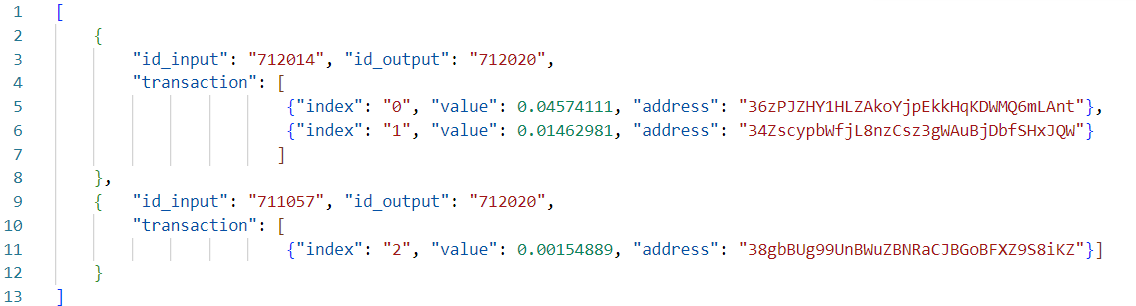
\includegraphics[keepaspectratio=true,scale=0.5]{Images/TX_JSON_BITVAS.png}
    \caption{Struttura del JSON usato per la rappresentazione delle Transazioni}
\end{figure}

\textit{id$\_$input} e \textit{id$\_$output} indicano il blocco di partenza e di arrivo del flusso legato alla transazione selezionata tramite interaccia grafica.
Le transazioni coinvolte in tale flusso sono identificate dall'array \textit{transaction}.

Infine per comprendere l'appartenenza di una transazione ad un determinato blocco, il sistema utilizza la struttura mostrata di seguito.


\begin{figure}[H]
    \centering 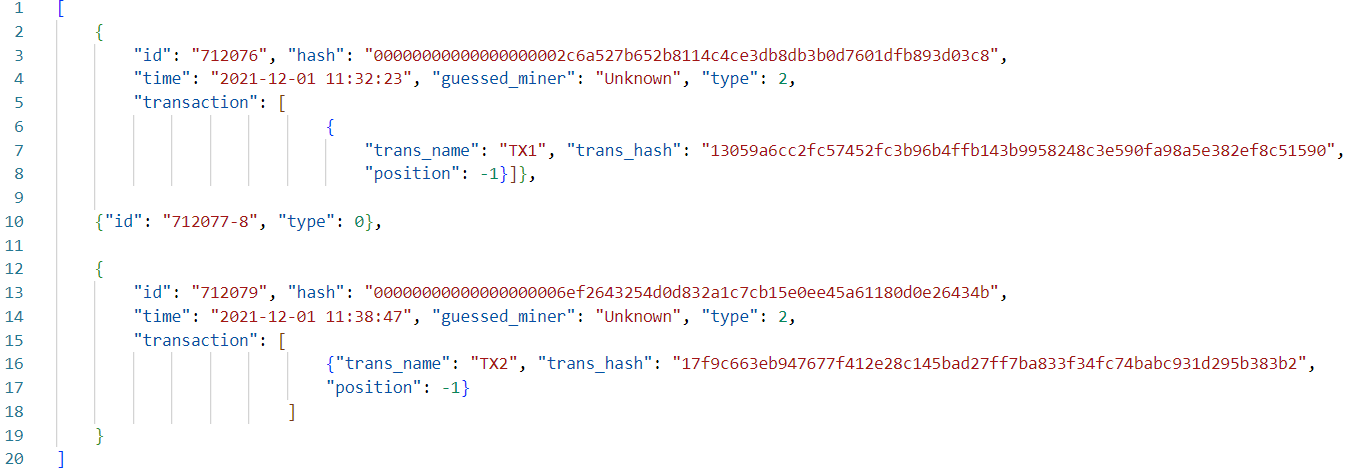
\includegraphics[keepaspectratio=true,scale=0.4]{Images/JSON_Definizione_TX.png}
    \caption{Struttura del JSON usato per il collegamento blocco-transazione}
\end{figure}

Per ogni blocco viene stilata una lista di transazioni validate al suo interno.
Nel caso in cui nella visualizzazione siano presenti dei blocchi, le cui transazioni non sono rilevanti, questi vengono semplificati tramite l'uso dei Cluster Block (riga 10).
BITVAS utilizza dei file ad hoc per le sue visualizzazioni.
Uno degli obiettivi cardine dell' API RESTful è la generazione dinamica di tali file partendo dai dati presenti all'interno del database a grafo.


\subsection{Architettura e diagramma di comunicazione}
Gli enormi vantaggi dell'architettura RESTful appurati in precedenza, la rendono la scelta migliore per lo sviluppo della API di questo progetto di tesi, la cui struttura e moduli sul quale si basa seguono il il seguente principio SRP.

\begin{center}
   \emph{``A module should be responsible to one, and only one, actor."} \cite{martin2018SoftwareStructure}
\end{center}
\thispagestyle{mystyle}
Il \emph{SRP (o Single-Responsibility-Principle)} \cite{PrinciplesOOD} \cite{martin2003agile} è uno dei principi fondamentali della programmazione orientata agli oggetti, il quale prevede che ogni modulo di un applicativo deve avere un solo motivo per essere modificato, ovvero una sola responsabilità , alla quale devono essere allineate tutte le funzionalità da essi offerte. Il motivo principale di tale principio è la diminuizione della complessità del progetto e il rischio di introdurre errori tramite la modifica del codice sorgente, aumentandone di conseguenza la scalabilità, la manutenibilità e la testabilità.
Per quanto concerne la programmazione di API, quanto detto si traduce nell'individuazione di endpoint specifici in grado di gestire dei task diversi e nella creazione di moduli completamente indipendenti l'uno dall'altro.

La struttura della API del progetto, infatti prevede quattro moduli separati, ognuno dei quali svolge un compito specifico: \emph{Index$\_$Server, JSON$\_$Controller, Query$\_$Controller, Request$\_$Controller}.

Index$\_$Server è il fulcro del middelware, pensato per occuparsi della gestione delle richieste da parte dei client e le corrispondenti risposte.
Con l'utilizzo delle tecnologie già citate permette al server di mettersi in ascolto di eventuali interrogazioni al database.

JSON$\_$Controller è un modulo utilizzato per la generazione dei file JSON strutturati in base ai dati richiesti.

Query$\_$Controller ha lo scopo di gestire e selezionare le varie query da inoltrare al server, a seconda delle necessità.

Request$\_$Controller è una classe utilizzabile dai client per poter integrare la API in altri applicativi.

\newpage
\thispagestyle{mystyle}
\begin{figure}[H]
    \centering 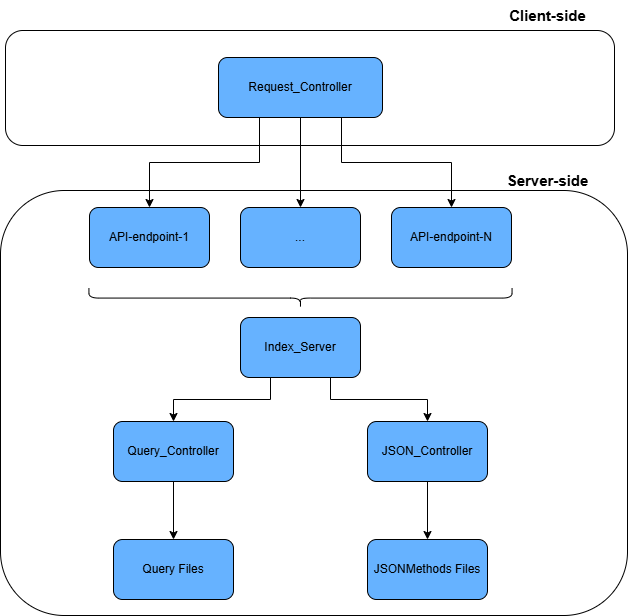
\includegraphics[keepaspectratio=true,scale=0.55]{Images/StrutturaInternaAPI.png}
    \caption{Struttura interna API}
\end{figure}

In figura 10 è mostrata la struttura interna della API, con tutti i moduli precedentemente elencati.
I due controller lato server, in base alle richieste, permettono di eseguire dei metodi finalizzati alla definizione delle query da inoltrare alla base di dati e quelli per la creazione dei JSON.
Tali metodi eseguono il codice sorgente di particolari moduli situati nelle cartelle \emph{Queries} e \emph{JSON methods}
L'indipendenza gli uni dagli altri di questi ultimi, permettono una gestione più semplice degli eventuali aggiornamenti futuri, legati allo sviluppo di nuove funzionalità.
Ad esempio se si volessero aggiungere altre visualizzazioni a BITVAS, si avrebbe la necessità di risucire ad estrapolare i dati necessari per generare le corrispettive risposte.
Per aggiornare il codice, basterebbe aggiungere i moduli per la query e la generazione dei file da inoltrare al client e modificare il codice dei controller, in modo da aggiungere dei metodi che permettano la gestione delle aggiunte effettuate.
Questa modularità fornisce maggior sicurezza in caso di modifica o aggiornamento del software, riducendo il rischio di errori.

\newpage
\thispagestyle{mystyle}
\begin{figure}[H]
    \centering 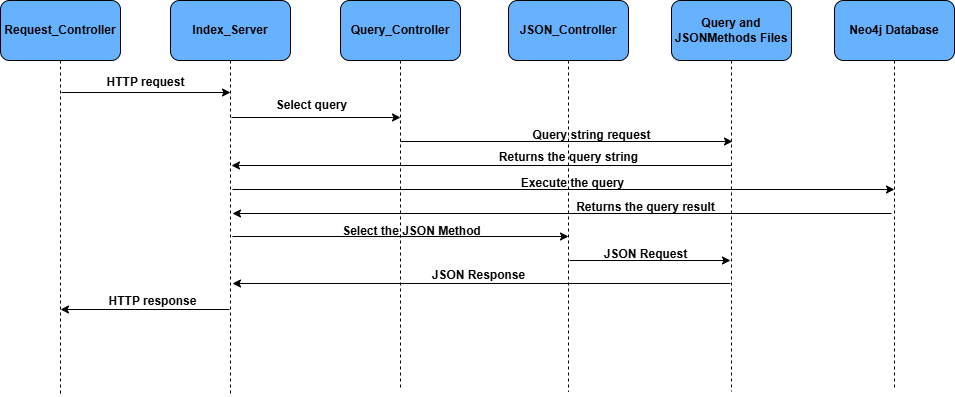
\includegraphics[keepaspectratio=true,scale=0.45]{Images/FlowChartAPI.png}
    \caption{Diagramma di sequenza della API}
\end{figure}

Attraverso il diagramma di sequenza mostrato in figura 11 è possibile individuare e comprendere nello specifico tutte le fasi della comunicazione tra i moduli dell'API RESTful sviluppata.

La prima fase consiste nell'inoltro da parte del client, tramite l'utilizzo di metodi specifici della classe Request$\_$Controller, di una richiesta HTTP verso il server.
Quest'ultimo, in attesa di interrogazioni, la gestisce come segue, tramite il file Index$\_$Server. A seconda dell'endpoint sollecitato e dei valori passati come parametri, attraverso l'utilizzo del modulo  Query$\_$Controller, viene estratta la query, sottoforma di stringa dal corrispondente file nella cartella Queries.
La stringa viene inviata al file Index$\_$Server, il quale la inoltra al database a grafo per poter estrapolare i dati necessari richiesti.
Il risultato delle query viene inoltrato al JSON$\_$Controller, tramite il quale si sceglie il metodo utile alla generazione dei file JSON,in grado di soddisfare le richieste del client, nella cartella JSONMethods.
Infine, questi ultimi vengono inviati al client, passando per la gesione di Index$\_$Server.

\subsection{Vantaggi architettura RESTful}

Presa in considerazione la natura dei due sistemi che si intende far interagire, l'architettura RESTful risulta la scelta più adeguata per lo sviluppo dell'API.
Quest'ultima infatti è molto efficace nel supporto di applicazioni web eseguite tramite browser, garantendo semplicità di utilizzo attraverso i metodi HTTP, ben conosciuti dagli sviluppatori. 

Inoltre grazie alla possibilità di utilizzare il protocollo HTTPS fornisce una maggiore sicurezza, proteggendo i dati durante il trasferimento.
Le informazioni possono essere trasferite dal server al client e viceversa attraverso molti formati di dati (JSON, XML, HTML, testo, ecc.), tutti indipendenti dalla piattaforma utilizzata, quindi interpretabili da ogni sistema operativo e da ogni dispositivo.

La leggerezza di questi formati combinata con la possibilià di memorizzare le risposte del server nella cache, garantisce un consumo minore della larghezza di banda rispetto ad altre soluzioni.

Infine grazie alla loro natura stateless e alla definizione di diversi endpoint per la gestione delle richieste, è possibile gestirne molte contemporaneamente.
La coesistenza di questi punti di forza permettono una gestione migliore del server, riducendone anche il carico computazionale, rendendo le API RESTful la scelta migliore per le web application.
\thispagestyle{mystyle}

\subsection{Endpoint}
Per garantire il Single-Responsibility-Principle di cui sopra, uno degli approcci fondamentali attuabili per quanto riguarda lo sviluppo di API è quello di identificare univocamente le risorse che possono essere richieste al server tramite la definizione di più endpoint, ognuno dei quali dedicato ad uno scopo specifico.
Più in dettaglio un endpoint è definibile come un URL  che funge da punto di interazione tra una API e un server, il quale si riferisce ad una singola risorsa.
I possibili parametri che è in grado di gestire si dividono in due tipi: \emph{in path} e  \emph{in query string}.
I parametri in path, utilizzati particolarmente per l'individuazione delle singole risorse, sono quelli che fanno parte dell'URL stesso.
Ad esempio, in \emph{https://urlexample.com/users/316704}, 316704 è un parametro nel percorso che potrebbe rappresentare l’ID di un utente.
Mentre quelli in query string, utili al filtraggio dei risultati di una richiesta, vengono aggiunti alla fine dell'URL dopo un 
punto interrogativo. Ad esempio, in  \emph{https://urlexample.com/search?q=books}, q=books è un parametro nella query string.

Tenendo conto della struttura dei dati necessari alla comunicazione del database di riferimento con \textit{BITVAS}, un endpoint che può essere definito riguarda l'estrapolazione delle informazioni per l'ottenimento delle visualizzazioni già sviluppate. L'identificazione di quest'ultimo avviene tramite l'URL \emph{http://localhost:7474/api/visualizations/:nomeVisual}.
 In questo caso si tratta di un endpoint che accetta richieste GET da parte dei client.
Uno dei parametri fondamentali è quello inserito nel percorso al posto di \emph{"nomeVisual"}, identificativo della visualizzazione che viene selezionata e della quale vengono prelevati i dati dal server, insieme al parametro \emph{"blockRef"} utile alla definizione del blocco centrale alle visualizzazioni progettate per \textit{BITVAS}.
Inoltre si può usufruire di un terzo parametro, ovvero \emph{"miner"}, necessario quando viene richiesta la MinerVisualization.

\newpage 
\begin{figure}[H]
    \centering 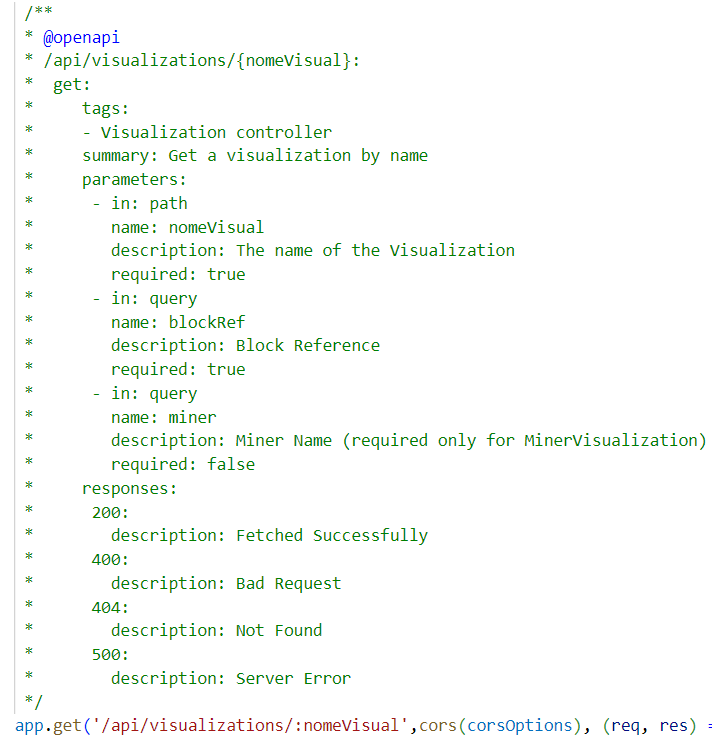
\includegraphics[keepaspectratio=true,scale=0.45]{Images/VisualizationEndpoint.png}
    \caption{Definizione endpoint tramite swagger UI e swagger-JSDocs}
\end{figure}

\thispagestyle{mystyle}

Oltre alla possibilità di estrazione dei dati necessari per il funzionamento del tool citato, L'\textit{API} mette a disposizione degli endpoint per permettere l'ottenimento di dati generici, utilizzabili in modi diversi a seconda delle esigenze.
Questi ultimi sono gestiti tramite l'URL  \\
\emph{http://localhost:7474/api/entities/:entityName}, il quale permette di ottenere i dettagli sulle entità presenti all'interno della base di dati.
Il parametro nel percorso \emph{"entityName"} identifica il tipo di entità, come transazioni, blocchi o i cluster progettati (hour, day, month e year). La selezione vera e propria di essa avviene con il timestamp attaverso il primo parametro in query string, ovvero \emph{"startTimestamp"}.
Se viene usato anche il parametro \emph{"endTimestamp"}, vengono estratti i dati di un insieme di entità, i cui timestamp sono compresi in un range temporale definito da entrambi i parametri.

Uno dei vantaggi dell'utilizzo dei database a grafo è quello di evidenziare le relazioni tra i dati presenti al suo interno, che in questo caso specifico pongono l'attenzione sui flussi di Bitcoin.
Per poter prelevare tali dati si può effettuare una richiesta all'URL 
 \\
 \emph{http://localhost:7474/api/flows/:ClusterToCluster}, dove \emph{"ClusterToCluster"} individua le entità coinvolte nel flusso da estrarre (es. DayToDay o BlockToYear). Con i parametri in query string \emph{"Timestamp"} e \emph{"RangeTimestamp"} si selezionano rispettivamente, il punto di arrivo e il range di partenza del flusso di Bitcoin.
Ad esempio utilizzando \textit{'2024-01-05'} e \textit{'2023-12-07T04,2023-12-07T09'}, vengono estrapolati i flussi uscenti dagli hour-cluster appartenenti al range definito che arrivano al day-cluster selezionato.

\subsection{Funzionalità progettate}
Le funzionalità progettate per la API riguardano nello specifico le tre categorie in linea con gli endpoint esposti.
Le prime utili all'interazione del database a grafo e BITVAS sono le seguenti:

\begin{itemize}
    \item \emph{getBlockVisualizationFirstPart(blockRef)} : Preso in input un riferimento al blocco, più precisamente un timestamp, restituisce la prima parte della BlockVisualization composta dai flussi di Bitcoin che partono da blocchi con timestamp ad una distanza temporale di massimo dodici ore e arrivano al blocco selezionato.

    \item \emph{getBlockVisualizationSecondPart(blockRef)} : Preso in input un riferimento al blocco, più precisamente un timestamp, restituisce la seconda parte della BlockVisualization composta dai flussi di Bitcoin partono dal blocco selezionato e arrivano ai blocchi con timestamp ad una distanza temporale di massimo dodici ore.

    \item 
    \emph{getCombinedVisualization(blockRef)}: Preso come parametro il timestamp identificativo del blocco centrale alla visualizzazione, restituire tutti i blocchi compresi nelle dodici ore precedenti e successive ad esso con tutte le relative relazioni, rappresentative dei flussi di Bitcoin. In questo caso i flussi fanno riferimento a tutti i blocchi compresi nell'arco temporale giornaliero.
\thispagestyle{mystyle}
    \item 
    \emph{getTXVisualizationFirstPart(hash)}: Preso in input un hash identificativo di una transazione, vengono restituite tutte le relazioni rappresentanti i flussi di Bitcoin in uscita ad essa.

    \item 
    \emph{getTXVisualizationSecondPart(hash)}: Preso in input un hash identificativo di una transazione, vengono restituite tutte le relazioni rappresentanti i flussi di Bitcoin in ingresso ad essa.
    
    \item 
    \emph{getMinerVisualizazion(blockRef, miner)}: Preso in input un timestamp identificativo del blocco centrale della visualizzazione e un miner specifico (es. Binance), restituisce tutti i flussi di Bitcoin riguardanti i blocchi compresi nelle dodici ore precedenti e successive al blocco scelto e che sono stati minati dallo stesso miner.
\end{itemize}

Per alcune visualizzazioni, come la BlockVisualization e la TXVisualization si è optato per la separazione in due funzioni distinte, per garantire un utilizzo più generale dei dati.
Infatti, questo è stato possibile soprattutto considerando la presenza nella loro struttura di un blocco sul quale viene concentrata l'attenzione per la rappresentazione dei flussi.
Questi ultimi, nei due casi sopra citati si dividono in due tipi, ovvero quelli che partono dal riferimento selezionato, e quelli che arrivano a tale elemento.

Come già trattato in precedenza, per permettere l'integrazione del database con altri applicativi in grado di porre il focus sui flussi temporali di Bitcoin.

\begin{figure}[H]
    \centering 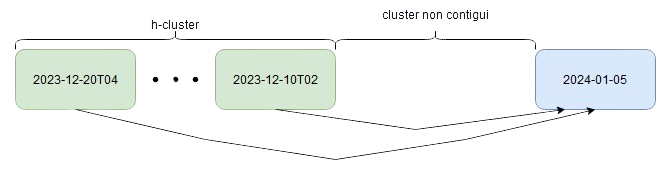
\includegraphics[keepaspectratio=true,scale=0.6]{Images/FlowsExampleQuery.png}
    \caption{Esempio di flusso tra hour cluster e day cluster}
\end{figure}

La rappresentazione può prevedere l'interazione tra cluster di tipo di verso che possono essere contigui e non. Per L'API sviluppata sono state definite le seguenti funzionalità:
\thispagestyle{mystyle}
\begin{itemize}

    \item \emph{getBlockToDayFlows(dClusterDate,BlocksTimestampRange)} : il primo parametro identifica il day cluster da prendere in considerazione (es. 2024-01-05), mentre il secondo sta ad indicare un insieme di blocchi, i cui timestamp sono compresi nel range \\ (es. 2024-01-05T03:56:00Z,2024-01-05T05:56:00Z).
    La funzione restituisce tutti i flussi di Bitcoin che partono dal range indicato e hanno come punto di arrivo il cluster selezionato.
    
    \item \emph{getHourToDayFlows(dClusterDate,hClusterRange)}:
    Preso in input un parametro identificativo di un day-cluster (es. 2024-01-05) e un range di timestamp che indicano un insieme di hour-cluster (es.  2024-01-05T03,2024-01-05T05), restituisce tutti i flussi di cryptovaluta che partono da questi ultimi e arrivano al day-cluster selezionato.
    
    \item \emph{getDayToDayFlows(dClusterDate,dClusterRange)} : in questo caso, vengono restituiti i flussi che partono e arrivano a cluster diversi della stessa tipologia. 
    \textit{dClusterDate} indica l'entità di arrivo dei flussi, mentre \textit{dClusterRange} rappresenta l'insieme dei cluster di partenza.

    
    \item \emph{getMonthToDayFlows(dClusterDate,mClusterRange)} : \emph{dClusterDate} individua il cluster di arrivo dei flussi di Bitcoin, mentre \emph{mClusterRange} indica un insieme di entità rappresentative dei mesi dai quali partono.
    
    \item \emph{getYearToDayFlows(dClusterDate,yClusterRange)} : restituisce i flussi di Bitcoin che partono dagli year-cluster, identificati tramite il parametro \emph{yClusterRange} (es. 2023,2024) e arrivano al dCluster selezionato tramite il primo parametro.
\end{itemize}

In questo caso vengono presi in considerazione i flussi di Bitcoin in entrata ai day-cluster, la cui struttura può essere ripetuta anche per gli altri cluster.

Oltre al focus ai suddetti flussi, l'API permette di poter estrarre dati generici riguardanti i dettagli delle entità presenti all'interno del database. Le funzioni sviluppate per tale scopo sono le seguenti : 

\begin{itemize}
    \item \emph{getTXInfo(startTimestamp,endTimestamp)} : restituisce le informazioni legate alle transazioni, il cui timestamp definito dal primo parametro.
    Il secondo parametro, ovvero \emph{endTimestamp} è opzionale e viene utilizzato nel caso in cui si vogliano conoscere i dati di transazioni comprese in un range di timestamp.

    \item \emph{getBlockInfo(startTimestamp,endTimestamp)} :
    restituisce i dettagli di un blocco nel caso in cui sia inizializzato solo il parametro \emph{startTimestamp}.
    Se viene definito anche il secondo parametro, vengono restituite tutte le informazione dei blocchi i cui timestamp sono compresi nell'intervallo temporale indicato dai due parametri.
    \item \emph{getXClusterInfo(startXTime,endXTime)} : è una generalizzazione delle funzioni programmate per il reperimento dei dettagli legati ai vari cluster nel database (es. \emph{getHClusterInfo} per gli hour-cluster)..
    Come per quelle precedenti, l'inizializzazione del solo primo parametro  permette di restituire i dati dei cluster identificati da esso.
    Nel caso in cui venga definito anche \emph{endXTime} vengono restituite le informazioni dei cluster appartenenti all'arco temporale indicato dai due parametri.
\end{itemize}
\thispagestyle{mystyle}
Tali funzioni sono strutturati in moduli separati e indipendenti tra loro, in modo da facilitare la manutenzione e l'aggiornamento del sistema, garantendo una maggiore scalabilità ed adattabilità a seconda delle esigenze.


\subsection{Moduli API}
In questa sezione vengono analizzati nel dettaglio i vari moduli dell'API sviluppata.
Le API sono componenti essenziali che permettono la comunicazione tra diversi applicativi, facilitando l'accesso e la manipolazione dei dati in modo efficiente e sicuro.
L'architettura modulare della API presentata in questa tesi è stata progettata con lo scopo di garantire scalabilità, manutenibilità e adattabilità del sistema.
Ogni modulo è stato sviluppato in modo da essere indipendente dagli altri con l'obiettivo di svolgere dei compiti specifici, riducendo la complessità di comprensione e modifica del codice sorgente.

\subsubsection{Index$\_$Server}
Index$\_$Server è il modulo principale dell'API, tramite il quale il server si mette in ascolto, su una determinata porta, in attesa di eventuali richieste da parte di possibili client.
Attraverso l'utilizzo di particolari moduli vengono definiti i parametri necessari alla connessione, tra cui anche le opzioni per a gestione del \emph{CORS(Cross-Origin Resource Sharing)}.

Il CORS \cite{CORS} è un meccanismo di sicurezza messo in atto dai browser in grado di permettere ai server di effettuare un controllo sulle risorse che possono essere richieste da un dominio diverso da quello in cui il server stesso è caricato.
La sua gestione risulta molto utile quando si ha a che fare con API il cui scopo è quello di accedere a risorse esterne come i database.
Inolte previene possibili attacchi malevoli nei quali un sito esterno potrebbe inviare richieste non autorizzate usando le credenziali degli utenti.


\begin{figure}[H]
    \centering 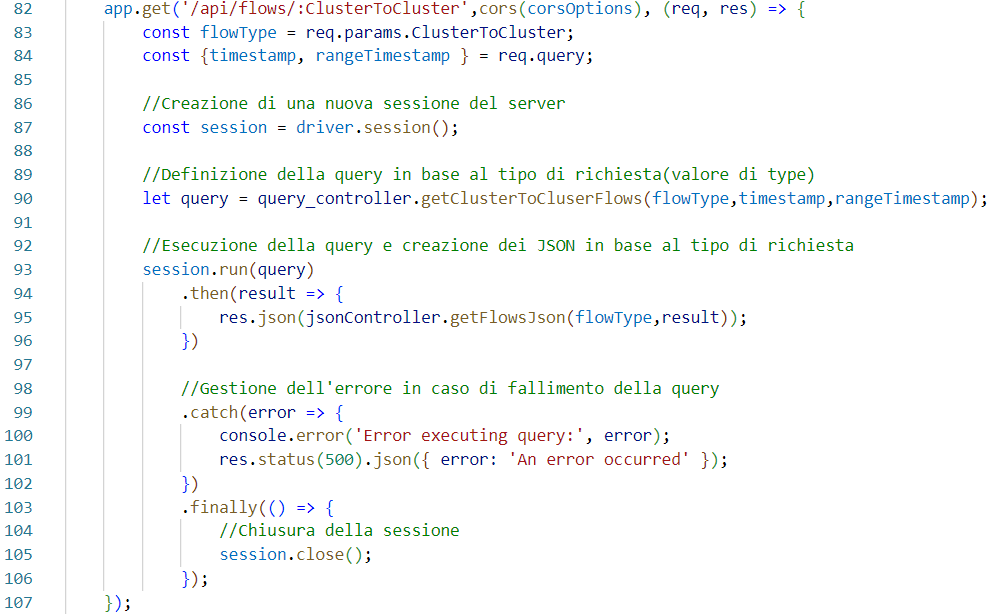
\includegraphics[keepaspectratio=true,scale=0.5]{Images/Index_Server_Endpoint.png}
    \caption{Definizione endpoint e gestione delle richieste}
\end{figure}

In figura 14 viene mostrato il codice sorgente riguardante l'inizializzazione di un endpoint, finalizzata tramite un'istanza del framework Express (riga 82), con i cui metodi è possibile definire il tipo di richieste che possono essere accettate (get,post,put,delete). Oltre alla scelta dell'URL identificativo dell'endpoint attraverso il quale si possono inoltrare richieste anche tramite browser, possono essere utilizzati altri parametri per ampliarne la gestione, come le opzioni per gestire il meccanismo CORS.

\thispagestyle{mystyle}
La gestione delle richieste avviene per fasi distinte.
In primis viene definita una sessione, tramite un'istanza dei driver di collegamento di neo4j, con il database a grafo sviluppato.
A seconda dell'endpoint a cui si fa riferimento, viene estrapolata la query da inoltrare tramite l'apposito controller, che successivamente viene inoltrata alla base di dati con l'istanza della connessione (riga 93).
Il risultato, gestito in modo asincrono, viene infine utilizzato per la creazione della risposta da inviare ai client, tramite il controller usato per la creazione dei JSON, previo eventuale controllo su possibili errori che possono verificarsi durante l'esecuzione. Al termine della gestione della richiesta la sessione al database viene chiusa.

Particolarmente importante è anche la gestione del caching, attuata con il modulo \emph{apicache} intallabile tramite npm, per permettere al server di gestire richieste ridondanti da parte del client, nell'arco di cinque minuti, in maniera tale da diminuire il carico sul server e velocizzare il reperimento dei dati lato client.

\subsubsection{Json$\_$Controller}
Il modulo JSON$\_$Controller è quello che si occupa di gestire la logica che intercorre tra il flusso di dati proveniente dal database e il client che ne richiede le informazioni, in modo da assolvere alla necessità di chiarezza nei dati e semplicità della struttura del sistema sviluppato garantendo tutti i principi precedentemente citati.
Si può considerare come il modulo centrale tramite il quale vengono effettuate delle scelte relative ai file JSON da generare, a seconda dei parametri utilizzati per la richiesta dei dati.
\thispagestyle{mystyle}
\begin{figure}[H]
    \centering 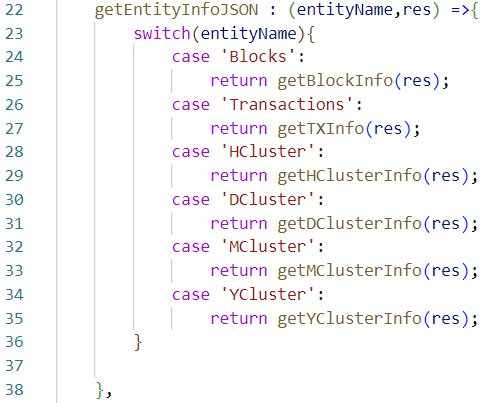
\includegraphics[keepaspectratio=true,scale=0.5]{Images/JSONControllerMethod.png}
    \caption{metodo JSON$\_$Controller per la scelta delle risposte da generare}
\end{figure}

In figura 15 è mostrata la scelta della struttura del file da inoltrare al client, in base alla richiesta ricevuta, legato alle informazioni delle entità presenti nella base di dati.
In questo caso a seconda del tipo di entità di cui si vogliono estrarre gli attributi, viene richiamato il modulo corrispondente al JSON da generare, nella cartella JSON Methods.

\subsubsection{Query$\_$Controller}
Il modulo Query$\_$Controller viene utilizzato come intermediario nella comunicazione tra il server e la cartella Queries contenente i file utilizzabili per l'estrapolazione delle query da inoltrare al database.
Come mostrato in figura 16, in base alla richiesta del client, distinguibile dai parametri inizializzati, viene estratta una query diversa, tramite i moduli importati.

\begin{figure}[H]
    \centering 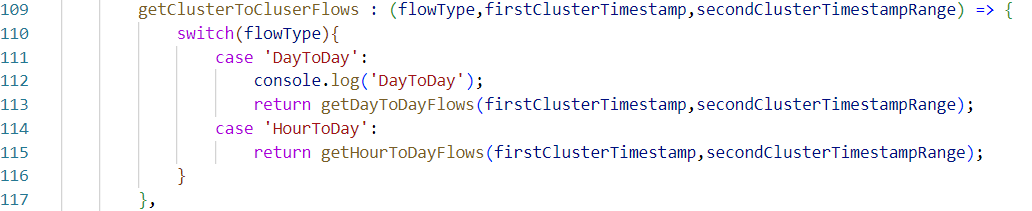
\includegraphics[keepaspectratio=true,scale=0.5]{Images/ExampleQueryControllerMethod.png}
    \caption{metodo Query$\_$Controller per l'estrazione delle query da inoltrare al database}
\end{figure}
\thispagestyle{mystyle}
Nel caso specifico mostrato, a seconda del tipo di entità coinvolte nel flusso richiesto viene estratta la Cypher query corrispondente. 

Per garantirne la corretta estrapolazione tramite l'utilizzo del modulo Request$\_$Controller, si occupa anche di individuare i tipi dei cluster coinvolti nei flussi, tramite l'apposito metodo getClusterType().
Quest'ultimo accetta come parametri in ingresso i timestamp dei cluster dei flussi che si vogliono estrarre, e restituisce il loro tipo 
(es. DClusterTimestamp se il timestamp è di un d-cluster), tramite i quali si hanno tutte le informazioni necessarie per definire la query string da inviare al server.
\subsubsection{JSONMethods Files e Query Files}

Per garantire scalabilità e manutenibilità del codice in linea con il principio SRP, si è deciso di sviluppare moduli indipendenti per l'estrapolazione delle query da inoltrare al database e per la generazione dei JSON, in modo che possano essere richiamati all'occorrenza dagli appositi controller.
In questo modo si facilita anche la comprensione del codice sorgente e si rende più semplice l'aggiunta di nuove funzionalità.
I file rappresentativi dei moduli si trovano nelle cartelle Queries e JSON Meethods e vengono importati nei moduli controller già trattati in precedenza.

\begin{figure}[H]
    \centering 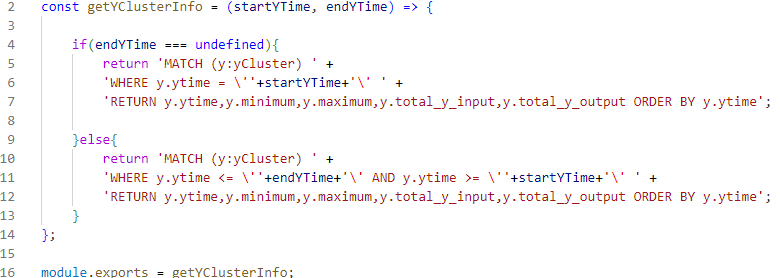
\includegraphics[keepaspectratio=true,scale=0.7]{Images/esempioModuliQuery.png}
    \caption{modulo per l'ottenimento della query getYClusterInfo()}
\end{figure}

\begin{figure}[H]
    \centering 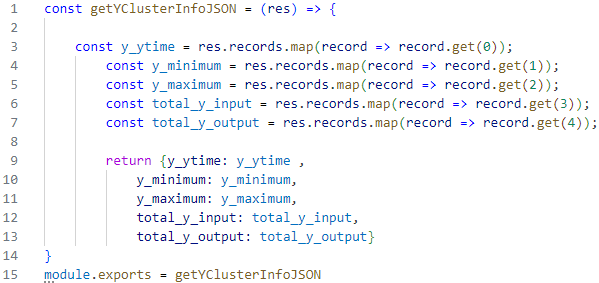
\includegraphics[keepaspectratio=true,scale=0.7]{Images/esempioModuliCreazioneJSON.png}
    \caption{modulo generazione JSON per la query getYClusterInfo()}
\end{figure}
\thispagestyle{mystyle}

\begin{onehalfspacing}
\subsubsection{Request$\_$Controller}
Il modulo Request$\_$Controller è di fondamentale importanza per garantire la comunicazione tra client e server, fungendo da interfaccia al database messo a disposizione.
Più nel dettaglio è una classe scritta in Javascript il cui unico attributo è un'istanza della classe XMLHttpRequest, che viene utilizzato per inoltrare le richieste HTTP al server, la cui query string viene definita a seconda del metodo richiamato e dai parametri utilizzati.

\thispagestyle{mystyle}

\begin{figure}[H]
    \centering 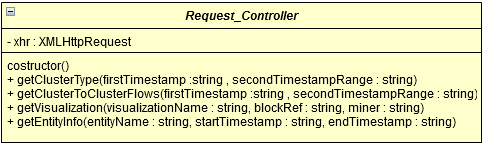
\includegraphics[keepaspectratio=true,scale=1]{Images/UMLRequestController.png}
    \caption{Diagramma UML della classe Request$\_$Controller}
\end{figure}

Quando viene richiamato il metodo per l'ottenimento dei flussi tra cluster, per identificarne il tipo viene fatto uso del metodo getClusterType, il quale prende come parametri i timestamp dei cluster e restituisce il loro tipo (es. una stringa contenente BlockTimestamp oppure HClusterTimestamp).
\end{onehalfspacing}

